\chapter{Evaluation}
\label{chap:evaluation}

In this chapter, we will conduct our evaluation in two parts. In the first part, we will evaluate the performance of different WebAssembly runtimes. In the second part, we will evaluate the performance of the WebAssembly-deployed functions compared to other non-WebAssembly functions.

\section{Goals}
\label{sec:goals}
%
Referring back to our research objectives from \autoref{sec:research-objectives}, the goals of this evaluation are to answer the following questions derived from the research question:
\begin{enumerate}
    \item What is the startup time of a simple \gls{WebAssembly} module?
    \item How do different programming languages compare?
    \item How do various runtimes compare to each other?
    \item How do the WebAssembly runtimes compare to native code?
    \item How does a WebAssembly-powered cloud platform measure up against a V8-powered cloud platform and a cloud platform with microVMs?
\end{enumerate}

\section{Methodology}
\label{sec:methodology}

To answer the above questions, we need to perform a series of different benchmarks. Each benchmark is targeted at answering a specific question. In \autoref{chap:runtimes}, we described the different runtimes with the corresponding compilation models, that we will be using in this evaluation. The next subsections will elaborate on the distinction between microbenchmarks and macrobenchmarks, as well as their application in answering the questions in \autoref{sec:goals}.

\begin{itemize}
    \item \textbf{Microbenchmarks}: Microbenchmarking is a technique used to measure the performance of a small function or a unit of code. It has the advantage of precisely measuring the performance of a specific function or code snippet. However, it can be difficult to extrapolate the results to a real-world scenario. Results from a specific scenario can look very different from the overall performance of a system. The evaluation does contain some microbenchmarks, but the main focus is on macrobenchmarks.
    \item \textbf{Macrobenchmarks}: Macrobenchmarking is not a well-defined term. It can be defined as a type of benchmark that measures the performance of a whole critical path. It is a more realistic approach to compare different systems with similar setups. The drawback of macrobenchmarks is that the results include the performance of the entire system, which is influenced by a lot of variables. To interpret the results, we will first try to subtract the noise and the system's overhead, and then we will compare the results with those of the microbenchmarks.
\end{itemize}

\section{Setup}
\label{sec:setup}

The evaluation setup consists of an AWS EC2 t2.medium instance, deployed on eu-central1 which is located in Frankfurt Germany. The instance is running Ubuntu 22.04 LTS with 2 vCPU and 4 GB of RAM. This instance is used to send requests and conduct benchmarks on different cloud platforms. The advantage of using a ec2 instance is the location. The latency between the ec2 instance and the cloud platforms is very low as shown in \autoref{fig:eval:setup}. The \gls{ICMP} packets have an average round-trip time of 1ms for Fastly, 1.35ms for Cloudflare, and 0.3ms for AWS, as the functions are served by a node in the same availability zone.

Additionally, we ran the benchmarks on this t2.medium instance to measure the runtime performance because it provides a comparable environment with the minimal required resources, to perform the runtime benchmarks. \autoref{fig:eval:setup} shows the deployment setup:

\begin{figure}[htbp]
    \centering
        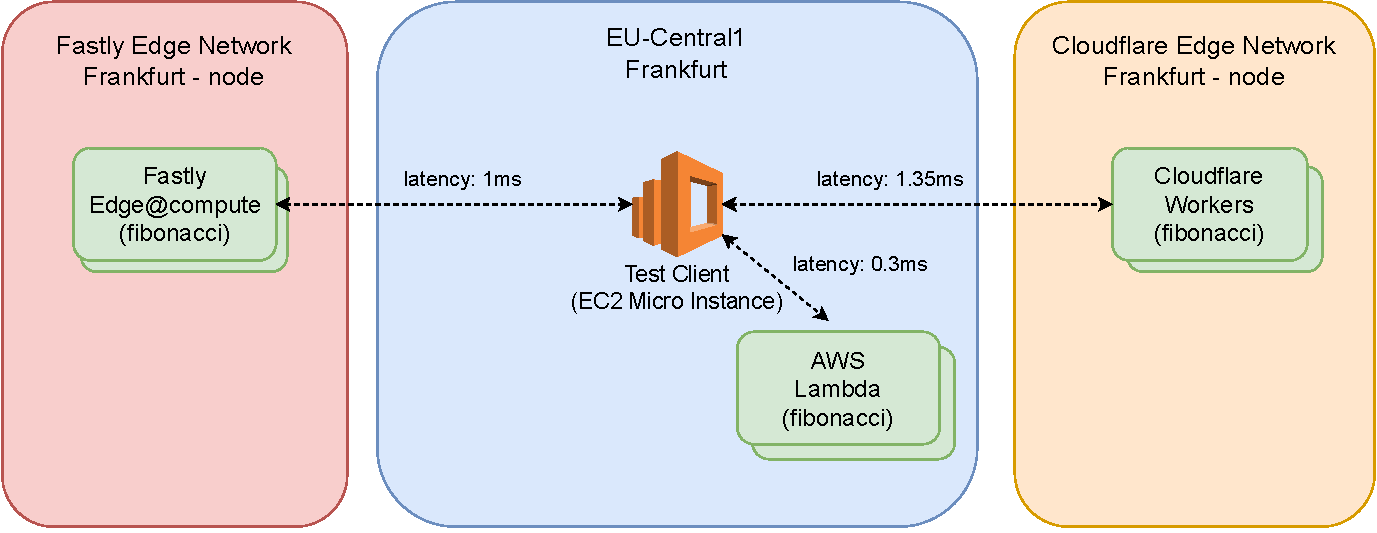
\includegraphics[width=1\linewidth]{images/evaluation/evaluation_setup.drawio.pdf}
    \caption{Deployment setup of the serverless functions}
    \label{fig:eval:setup}
\end{figure}

Moreover, we used a MacBook Pro with M1 Pro CPU and 32GB of RAM to run the runtime benchmarks locally. The benchmarks were executed while the MacBook was plugged into the power supply, and no other major processes were running during the benchmarking process. The M1 Pro CPU is an ARM-based CPU, which is different from the t2.medium's Intel x86 CPU. The results of the two setups cannot be compared directly, but we can use them as a high-level comparison to inspect factors like CPU architecture compatibility and identify any significant outliers. We have tried to perform the benchmarks on a Raspberry PI 2, but the ARM 32-bit architecture is not supported by runtimes like Wasmtime and Wasmer. Aside from that, we also tried a more limited setup with t2.micro instance, but the benchmark code did not compile in a reasonable time. The t2.medium instance is the smallest instance that can run the benchmarks in a reasonable time. 

\section{Criterion}
\label{sec:criterion}

Criterion.rs \cite{heisler_2023_criterionrs} is a statistics-driven benchmarking library for Rust. In our evaluation, Criterion is used to measure the performance of different runtimes. Criterion is a powerful tool that can be employed to measure the performance of a function or a code snippet. Criterion.rs is inspired by Haskell's criterion library. The library provides HTML reports with statistical analysis of the benchmark results, including the mean, median, standard deviation, as well as the regression with previous runs. Moreover, we utilize the library's utility functions such as \texttt{black\_box} to prevent the compiler from optimizing the code away.

Criterion process consists of four phases:

\begin{itemize}
    \item \textbf{Warmup}: In the warmup time the routine is repeatably executed for a given time. This gives the CPU, OS caches and also the JIT compiler if present, time to adapt and optimize the code.
    \item \textbf{Measurement}: Similar to the warmup time the code is repeatably executed in this phase, but unlike the warmup time, the measurement results will be used for analysis. The measurements consists of many samples. Each sample has one or multiple iteration of routines. 
    \item \textbf{Analysis}: This is the phase where the statistical analysis is performed. Values outside of the 25th and 75th percentile are classified as outliers. Values outside of the 5th and 95th percentile are classified as severe outliers. The mean, median, standard deviation, and the regression metrics with previous runs are calculated in this phase.
    \item \textbf{Comparison}: In this phase the statistics of the current run are compared to the previous runs. The comparison is performed using a regression analysis. The results of the comparison are shown in the HTML report and in console output.
\end{itemize}

\section{Benchmarks}
\label{sec:benchmarks}

In this section, we will perform the benchmarks that address the questions outlined in \autoref{sec:goals}. The benchmarks are split into two categories: \textit{runtime} and \textit{serverless platform}. Under the \textit{runtime} category, we will measure the "cold start" time and conduct performance tests with various workloads. In the \textit{serverless platform} category, we will benchmark the response time and compare the performance of different platforms.

\subsection{Cold Start - Instantiation}
\label{subsec:cold-start}

One of the challenges of this thesis has been to precisely define what "cold start" means and how to measure it. In the context of WebAssembly, we define "cold start" as the time it takes from creating a runtime context to loading the module and executing the module's "start" function. This definition is specifically applicable to WebAssembly and V8 setups. The reason for this specificity is the difference between the WebAssembly runtime and a virtualized solution like Firecracker's microVM, which powers the Lambda and AWS Fargate instances. In a virtualized solution, the "cold start" time is the time it takes to boot the virtual machine and load the application. In the case of WebAssembly, the runtime is already running, and the module is loaded into the runtime.

As mentioned before, we utilized the criterion library to measure the instantiation process. Initially, we created a \textit{WAT} file (as shown in \autoref{lst:eval-small-memory}) that included a small memory and a "start" function. The benchmark was executed both locally and on a t2.medium instance. The results are illustrated in \autoref{fig:bench:instantiation:empty-wasm}.

\begin{lstlisting}[frame=lines, style=Wasm, caption={WASI module with small memory}, showstringspaces=false, captionpos=b, label={lst:eval-small-memory}]
    (module
        (memory 1)
        (func (export "_start"))
    )
\end{lstlisting}

\begin{figure}[htbp]
    \centering
        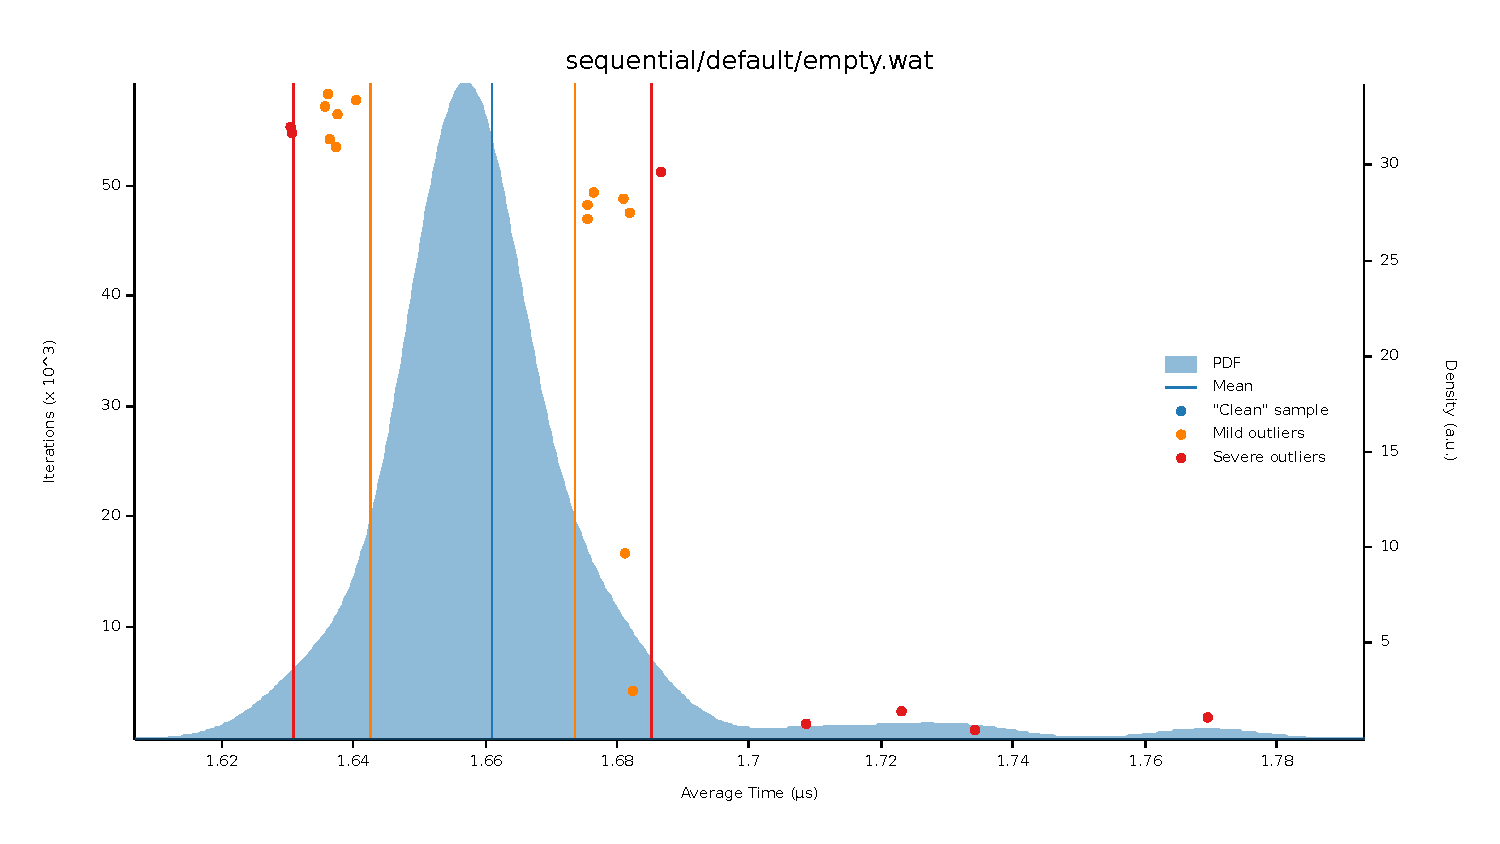
\includegraphics[width=1\linewidth]{images/benches/sequential_default_empty_wasm.pdf}
    \caption{Instantiation distribution of an empty Wasm module with Wasmtime and M1 Pro CPU}
    \label{fig:bench:instantiation:empty-wasm}
\end{figure}

Furthermore, we also conducted an instantiation benchmark, where we first compiled a simple Rust "Hello World" program to a WASI module and then instantiated it using Wasmtime. The results of this benchmark are shown in \autoref{fig:bench:instantiation:wasi}. Please note that we did not measure the compilation time.

Additionally, we performed another benchmark where we defined a \textit{WAT} file with a large data segment and memory. The results for this benchmark are included in the appendix section.

\begin{figure}[htbp]
    \centering
        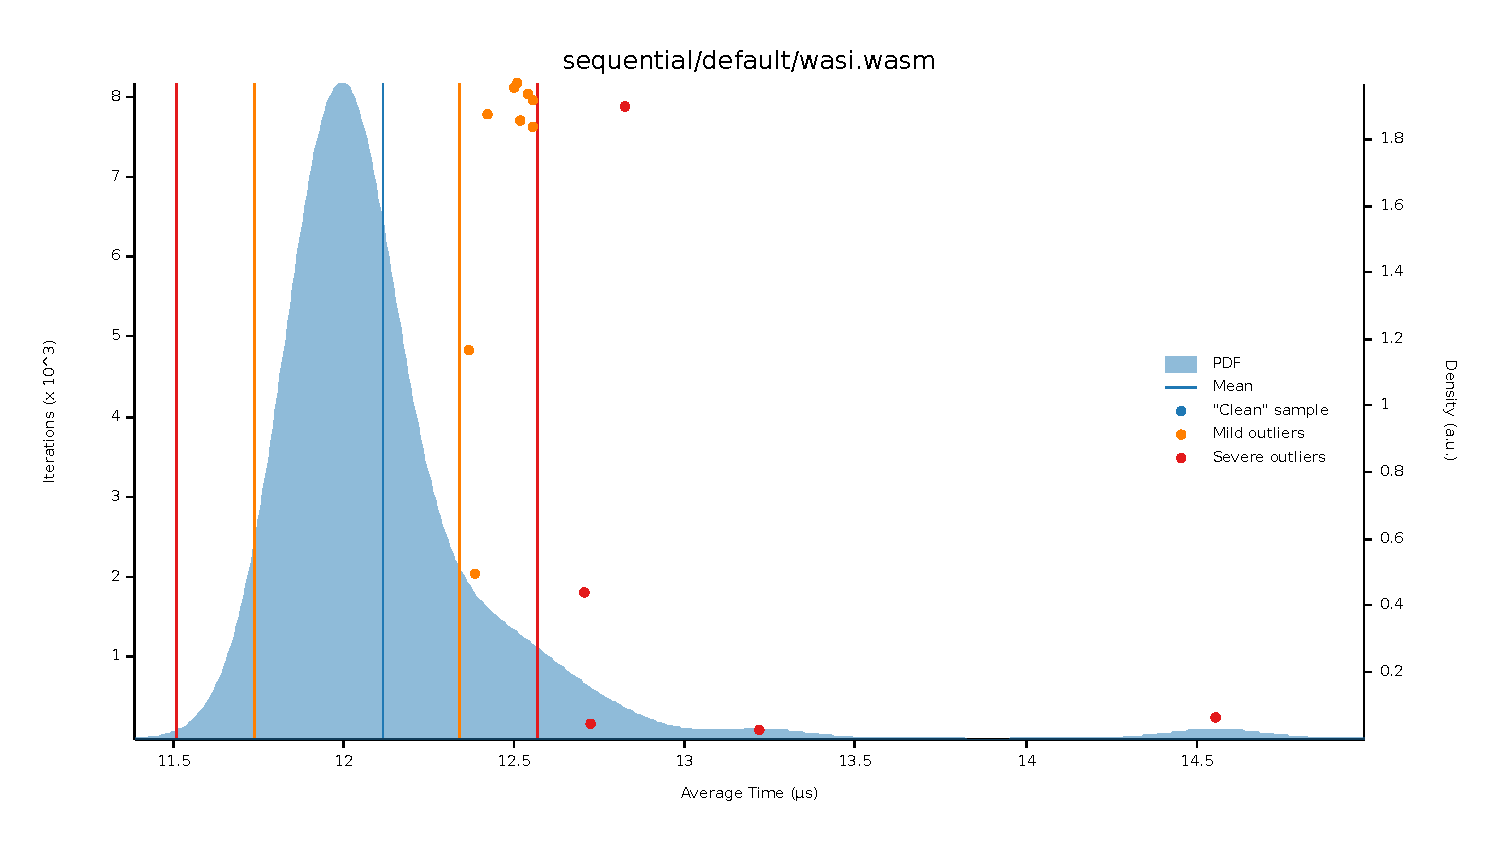
\includegraphics[width=1\linewidth]{images/benches/sequential_default_wasi.pdf}
    \caption{Instantiation distribution of a WASI module with Wasmtime and M1 Pro CPU}
    \label{fig:bench:instantiation:wasi}
\end{figure}


\subsection{Execution Performance}
\label{subsec:executation-performance}

In this section, we will assess the execution performance of different runtimes. Once again, we will use the criterion library for analysis. For this evaluation, we have created both an executable binary and an executable Wasm module. Both the native binary and the Wasm module contain the benchmark function. To ensure realistic production performance, we compiled with the \texttt{--release} flag. Moreover, the Wasm module was automatically optimized using \texttt{wasm-opt}. During benchmarking, the criterion's \texttt{black\_box} utility is used to prevent the compiler from optimizing the code away.

For this evaluation, we have chosen the following runtimes: Wasmtime and Wasmer as the JIT runtimes, Wasm3 as the interpreter runtime, and WasmEdge as the AOT runtime. The benchmarks were conducted using the following functions:

\subsubsection{Fibonacci}

The Fibonacci function is a well-known benchmark used to assess the performance of a runtime. It is chosen for two main reasons: Firstly, it involves a recursive computation, making it a CPU-intensive task. Secondly, it is a simple function that can be easily understood and implemented in any environment.

\subsubsection{Blake3}

Blake3 is an efficient and fast cryptographic hash function. With the increasing use of cryptographic functions in modern applications, it becomes important to measure the performance of such functions. As a deterministic one-way function, Blake3 hashes a "Hello World" string in the benchmark. Unlike the Fibonacci function, Blake3 is expected to execute much faster, leading us to assume that an interpreter runtime or an AOT runtime may have an advantage over a JIT runtime. 

The results of this evaluations are shown in \autoref{fig:eval:t2medium-fib_40}, \autoref{tab:t2-medium-fibonacci} and \autoref{tab:blake3}. We will discuss the results in \autoref{sec:discussion}.

\begin{figure}[htbp]
    \centering
        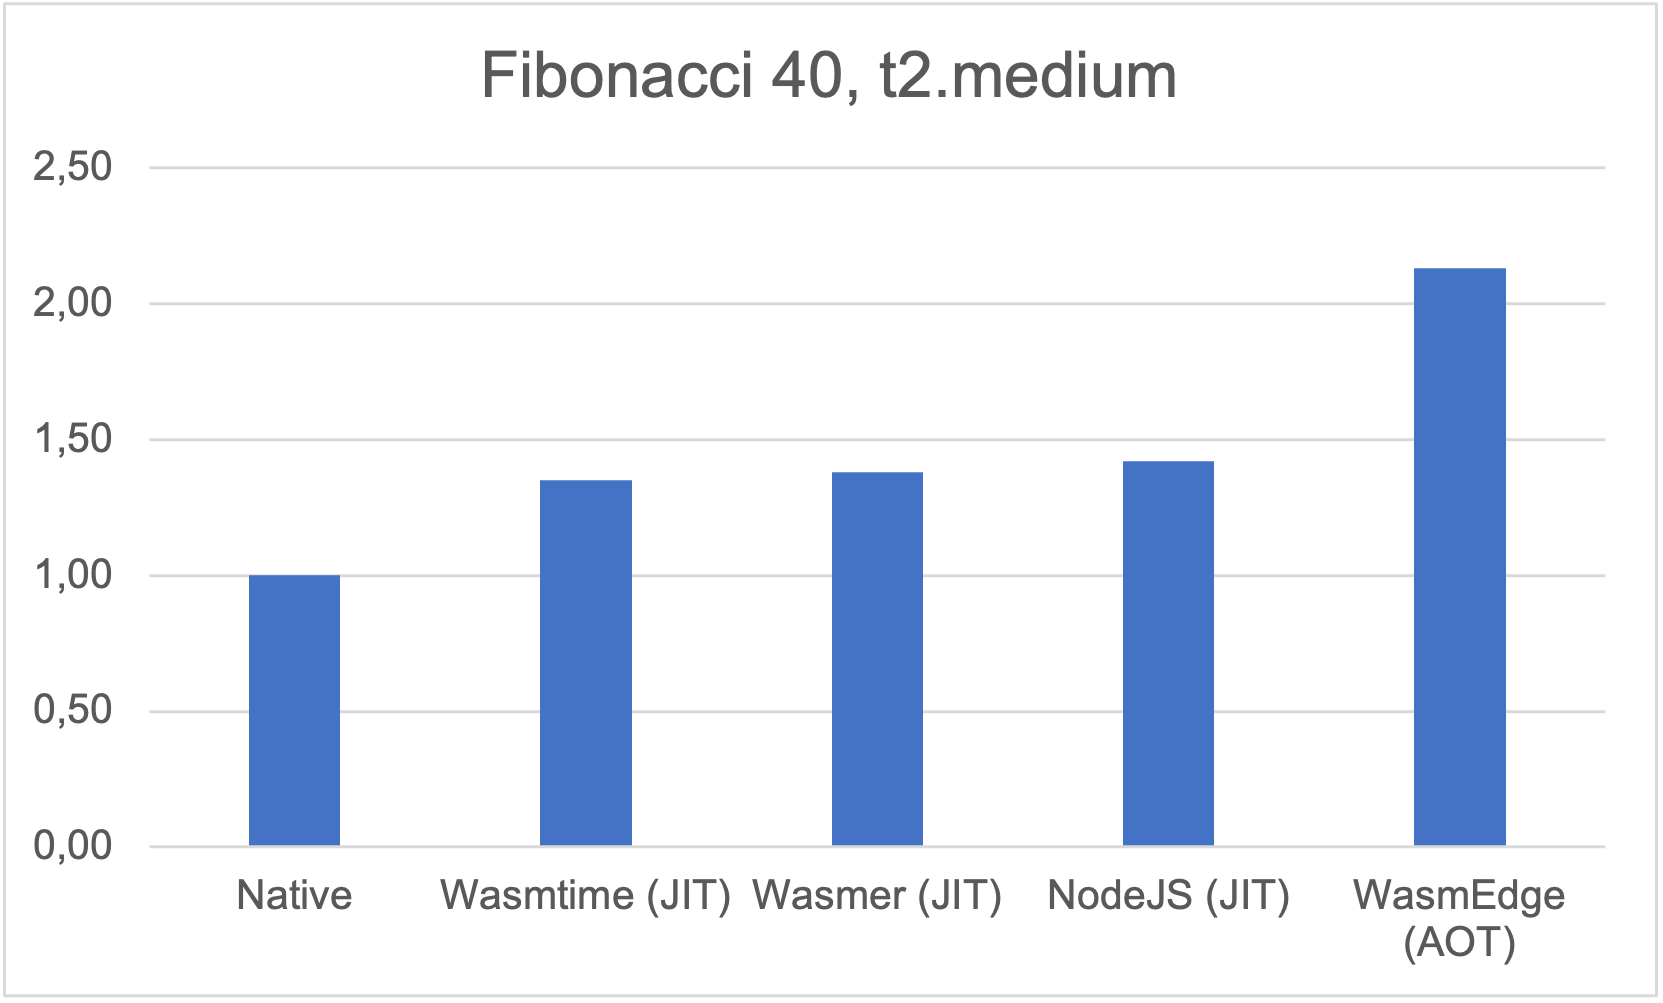
\includegraphics[width=1\linewidth]{images/benches/t2medium_fib_40.png}
    \caption{Runtime comparison on t2.medium: Fibonacci 40 results, excluding Wasm3}
    \label{fig:eval:t2medium-fib_40}
\end{figure}

\begin{table}[]
    \begin{tabular}{|lll|l|lll|}
    \cline{1-3} \cline{5-7}
    \multicolumn{3}{|c|}{\textbf{Fibonnaci 40, t2.medium}}                                           & \multirow{8}{*}{} & \multicolumn{3}{c|}{\textbf{Fibonnaci 32, t2.medium}}                                           \\ \cline{1-3} \cline{5-7} 
    \multicolumn{1}{|l|}{\textbf{Runtime}}  & \multicolumn{1}{l|}{\textbf{Baseline}} & \textbf{Time} &                   & \multicolumn{1}{l|}{\textbf{Runtime}}  & \multicolumn{1}{l|}{\textbf{Baseline}} & \textbf{Time} \\ \cline{1-3} \cline{5-7} 
    \multicolumn{1}{|l|}{\textbf{Native}}   & \multicolumn{1}{l|}{1.00}              & 396.1±0.42ms  &                   & \multicolumn{1}{l|}{\textbf{Native}}   & \multicolumn{1}{l|}{1.00}              & 9.11±0.02ms   \\ \cline{1-3} \cline{5-7} 
    \multicolumn{1}{|l|}{\textbf{Wasmtime}} & \multicolumn{1}{l|}{1.35}              & 534.74±2.24ms &                   & \multicolumn{1}{l|}{\textbf{Wasmtime}} & \multicolumn{1}{l|}{1.31}              & 11.92±1.56ms  \\ \cline{1-3} \cline{5-7} 
    \multicolumn{1}{|l|}{\textbf{Wasmer}}   & \multicolumn{1}{l|}{1.38}              & 546.61±2.61ms &                   & \multicolumn{1}{l|}{\textbf{Wasmer}}   & \multicolumn{1}{l|}{1.33}              & 12.1±1.74ms   \\ \cline{1-3} \cline{5-7} 
    \multicolumn{1}{|l|}{\textbf{NodeJS}}   & \multicolumn{1}{l|}{1.42}              & 562.46±2.41ms &                   & \multicolumn{1}{l|}{\textbf{NodeJS}}   & \multicolumn{1}{l|}{1.45}              & 13.2±2.56ms   \\ \cline{1-3} \cline{5-7} 
    \multicolumn{1}{|l|}{\textbf{WasmEdge}} & \multicolumn{1}{l|}{2.13}              & 843.69±4.21ms &                   & \multicolumn{1}{l|}{\textbf{WasmEdge}} & \multicolumn{1}{l|}{2.21}              & 20.11±3.23ms  \\ \cline{1-3} \cline{5-7} 
    \multicolumn{1}{|l|}{\textbf{Wasm3}}    & \multicolumn{1}{l|}{4.82}              & 1909.2±8.52ms &                   & \multicolumn{1}{l|}{\textbf{Wasm3}}    & \multicolumn{1}{l|}{4.51}              & 41.04±2.51ms  \\ \cline{1-3} \cline{5-7} 
    \end{tabular}
    \caption{Runtime Benchmark: Fibonacci 40 and 32 on t2.medium; Wasmtime, Wasmer, NodeJS (JIT), WasmEdge (AOT), Wasm3 (Interpreter)}
    \label{tab:t2-medium-fibonacci}
\end{table}


\begin{table}[]
    \begin{tabular}{|lll|l|lll|}
    \cline{1-3} \cline{5-7}
    \multicolumn{3}{|c|}{\textbf{Blake3, M1 PRO CPU}}                                                & \multirow{8}{*}{} & \multicolumn{3}{c|}{\textbf{Blake3, t2.medium}}                                                  \\ \cline{1-3} \cline{5-7} 
    \multicolumn{1}{|l|}{\textbf{Runtime}}  & \multicolumn{1}{l|}{\textbf{Baseline}} & \textbf{Time} &                   & \multicolumn{1}{l|}{\textbf{Runtime}}  & \multicolumn{1}{l|}{\textbf{Baseline}} & \textbf{Time}  \\ \cline{1-3} \cline{5-7} 
    \multicolumn{1}{|l|}{\textbf{Native}}   & \multicolumn{1}{l|}{1.00}              & 83.8±1.86ns   &                   & \multicolumn{1}{l|}{\textbf{Native}}   & \multicolumn{1}{l|}{1.00}              & 114.7±0.19ns   \\ \cline{1-3} \cline{5-7} 
    \multicolumn{1}{|l|}{\textbf{NodeJS}}   & \multicolumn{1}{l|}{1.10}              & 92.3±2.24ns   &                   & \multicolumn{1}{l|}{\textbf{NodeJS}}   & \multicolumn{1}{l|}{1.32}              & 150.084±1.56ns \\ \cline{1-3} \cline{5-7} 
    \multicolumn{1}{|l|}{\textbf{Wasmtime}} & \multicolumn{1}{l|}{1.13}              & 94.3±2.61ns   &                   & \multicolumn{1}{l|}{\textbf{Wasmtime}} & \multicolumn{1}{l|}{1.41}              & 161.727±1.74ns \\ \cline{1-3} \cline{5-7} 
    \multicolumn{1}{|l|}{\textbf{Wasmer}}   & \multicolumn{1}{l|}{1.35}              & 113.13±2.41ns &                   & \multicolumn{1}{l|}{\textbf{Wasmer}}   & \multicolumn{1}{l|}{1.46}              & 167.462±2.56ns \\ \cline{1-3} \cline{5-7} 
    \multicolumn{1}{|l|}{\textbf{WasmEdge}} & \multicolumn{1}{l|}{2.05}              & 171.5±4.21ns  &                   & \multicolumn{1}{l|}{\textbf{WasmEdge}} & \multicolumn{1}{l|}{2.15}              & 246.605±3.23ns \\ \cline{1-3} \cline{5-7} 
    \multicolumn{1}{|l|}{\textbf{Wasm3}}    & \multicolumn{1}{l|}{4.82}              & 403.91±8.52ns &                   & \multicolumn{1}{l|}{\textbf{Wasm3}}    & \multicolumn{1}{l|}{4.97}              & 570.059±2.51ns \\ \cline{1-3} \cline{5-7} 
    \end{tabular}
    \caption{Runtime Benchmark: Blake3 on M1 PRO and t2.medium; Wasmtime, Wasmer, NodeJS (JIT), WasmEdge (AOT), Wasm3 (Interpreter)}
    \label{tab:blake3}
\end{table}

\subsection{Evaluating Serverless Platforms}
\label{subsec:evaluating-serverless-platforms}

Evaluating various serverless platforms is a challenging task, because there are a handful of variable factors that can influence the measurements.

We deployed the same functions on different platforms and with different programming languages. The functions were invoked by a timestamp in order to prevent caching of the response by the CDN. The functions were invoked sequentially with a delay of 15 minutes between each invocation. The delay was chosen to prevent warm starts, we conducted a few tests to find the idle time before the functions are terminated. A bash script was used to invoke the functions with curl and write the response metrics into a file. As mentioned in the \autoref{sec:setup} the test instance has a latency of 0.3 to 1.3 milliseconds to the functions. Here is a list of the deployed functions:

\begin{itemize}
    \item \textbf{Fibonacci}: The Fibonacci function calculates the Fibonacci for a given number \textit{n}. The function is implemented in Rust, JavaScript and Go. We deployed the function on Fastly Compute@Edge, Cloudflare Workers (only JavaScript) and AWS Lambda (only JavaScript).
    \item \textbf{Blake3}: The Blake3 function calculates the hash of a given string. We used the string "Hello World". The function is implemented in Rust, JavaScript and Go. We deployed the function on Fastly Compute@Edge, Cloudflare Workers (only JavaScript) and AWS Lambda (only JavaScript).
\end{itemize}

\subsubsection{Curl Performance Metrics}

The curl command is a powerful built-in tool in the bash shell. We use it to send the requests from the test client to each serverless function. An overview of how a request is sent and what processes are involved is shown in \autoref{fig:eval:curl-metrics}. The curl command is executed with the following parameters:
\texttt{curl -w "@curl-format.txt" -o /dev/null -s "https://serverless-function-address.app/"}

the \texttt{curl-format.txt} formats the response. The following metrics are recorded (more details on \cite{speedtestdemon_2021_cheat}):

\begin{itemize}
    \item \textbf{time\_namelookup}: The time in seconds it took from the start until domain resolving was completed.
    \item \textbf{time\_connect}: The time in seconds it took from the start until the three way handshake was completed from the clients perspective.
    \item \textbf{time\_appconnect}: Is the time where the TLS setup is done. The client is able to send the HTTP GET request.
    \item \textbf{time\_starttransfer}: The time it took until the first byte of the response was by curl. This is also known as the TTFB (Time to first byte). If we calculate \texttt{TTFB - (time\_connect - time\_namelookup)} then we get the time it took for the server to process the request.
    \item \textbf{time\_total}: The total time in seconds is the duration between the time the request was sent and the time the last byte of the response was received.
\end{itemize}

These metrics provide valuable insights into the actual performance of the serverless functions and analyze the outliers caused by the network.


\begin{figure}[htbp]
    \centering
        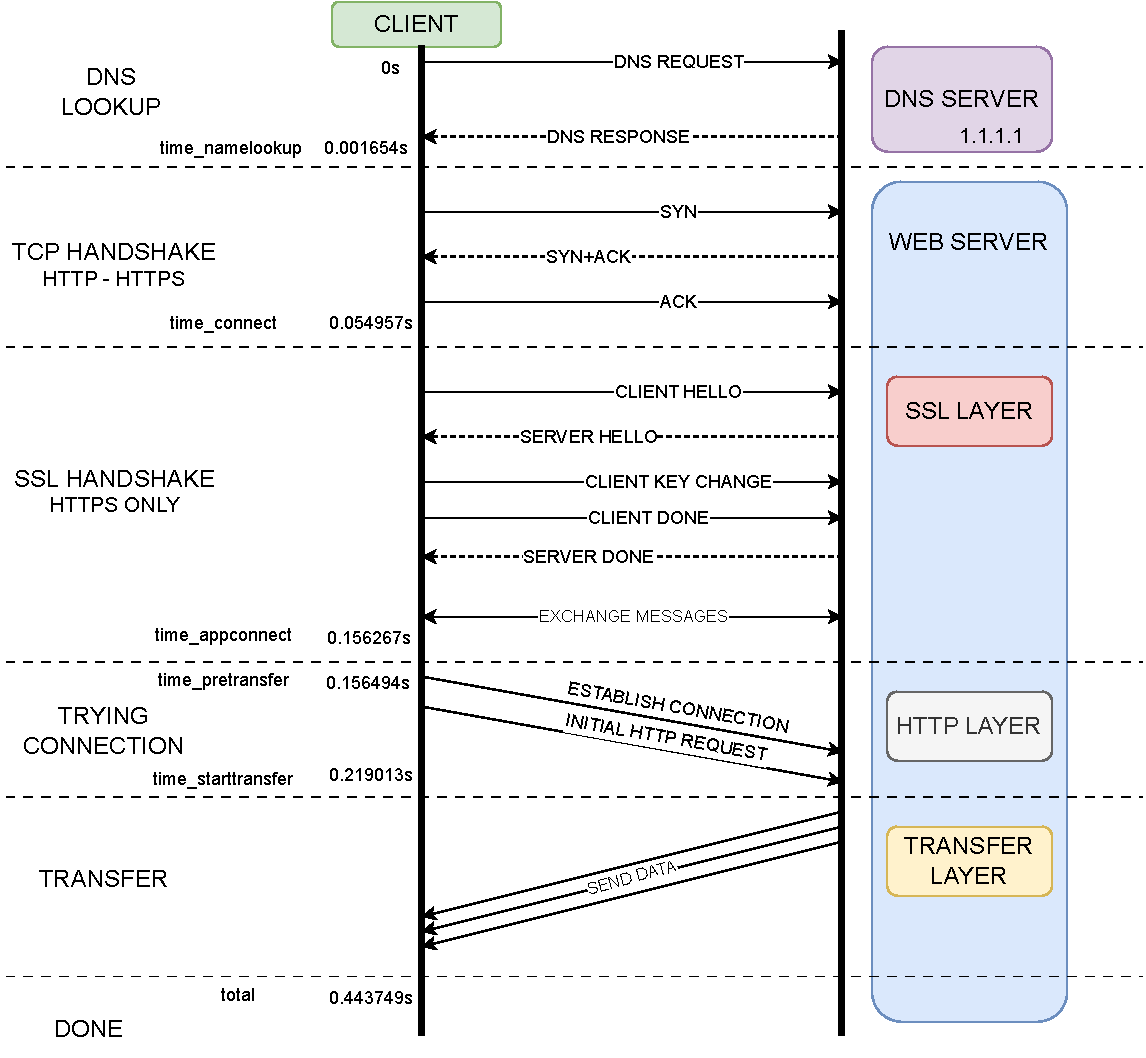
\includegraphics[width=1\linewidth]{images/evaluation/curl_performance_metrics.drawio.pdf}
    \caption{Curl performance metrics visualization, redrawn from \cite{speedtestdemon_2021_cheat}}
    \label{fig:eval:curl-metrics}
\end{figure}

\begin{figure}[htbp]
    \centering
        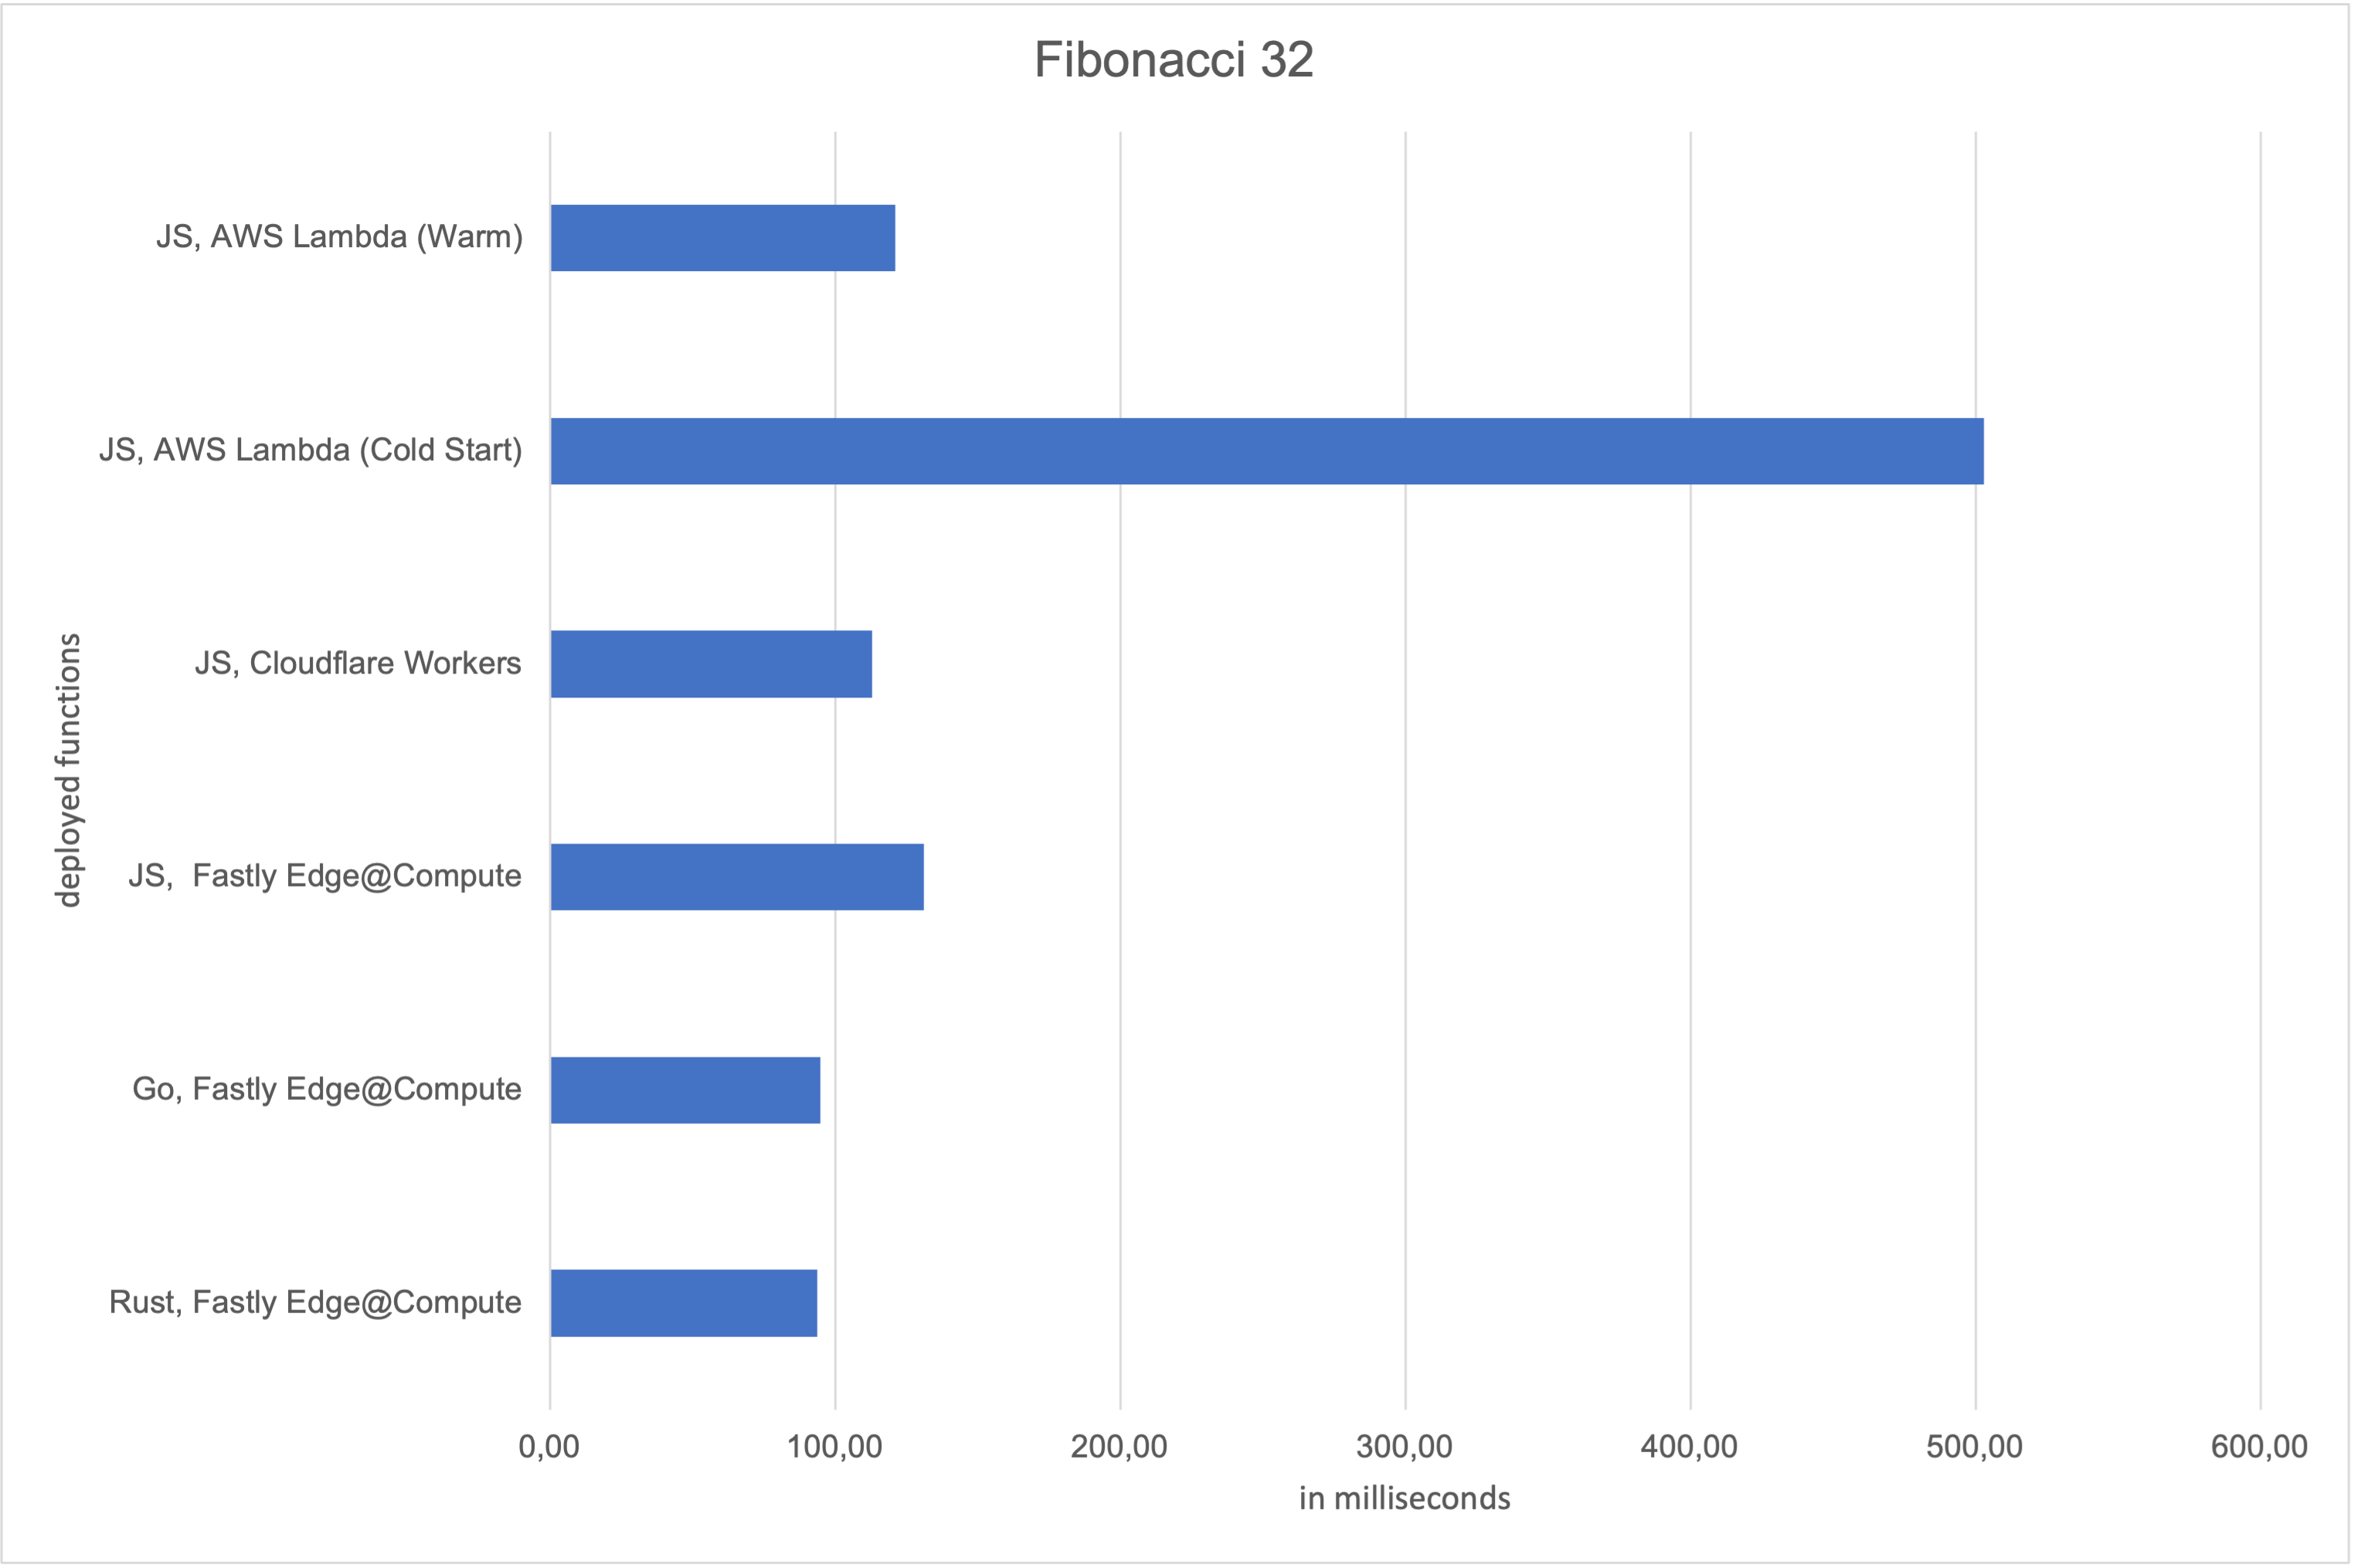
\includegraphics[width=0.95\linewidth]{images/benches/deployed_functions_fib32.png}
    \caption{Derived results of deployed functions: Fibonacci 32, the result is calculated with TTFB - (time connect - time namelookup)}
    \label{fig:eval:deployed-functions}
\end{figure}

\section{Discussion}
\label{sec:discussion}

In this section we will answer the questions from \autoref{sec:goals} and discuss the findings of the evaluation. We will also address the limitations encountered during the evaluation.

\subsection{Evaluation Questions}

\textbf{1. What is the startup time of a simple \gls{WebAssembly} module?}

We evaluated the startup time of a simple \textit{WAT} file, loading a Rust to \gls{wasi}-compiled file, and a Wasm module with a large data segment. These benchmarks, as shown in \autoref{fig:bench:instantiation:wasi}, indicate a startup time ranging from 5 to 40 microseconds overall. Additionally, we evaluated the startup time of deserializing and loading a deserialized Wasm module. The startup time of a deserialized Wasm module is about 98 microseconds for a t2.medium instance (shown in \autoref{fig:bench:instantiation:t2-deserialize-wasi-wasm} in the appendix). Under adverse conditions, we could see a startup time of 1 to 5 milliseconds depending on the size of the Wasm module. The size of a bundled serverless function is typically small, and some cloud providers impose size limits.

\textbf{2. How do different programming languages compare?}

We evaluated the performance of the programming languages Rust, JavaScript, and Go. The performance of these programming languages is similar, with Rust being slightly faster than Go and JavaScript, as shown in \autoref{fig:eval:deployed-functions}.

\textbf{3. How do various runtimes compare to each other?}

The results show that Wasmtime and Wasmer are similar in performance, with Wasmtime being slightly faster than Wasmer. In contrast, Wasm3, as shown in \autoref{tab:blake3}, is the slowest runtime in our evaluation. It is not surprising that Wasm3 is slower than Wasmtime and Wasmer, as Wasm3 is an interpreter runtime with a main focus on small footprint and portability. Wasm3 can find its use case in embedded systems, where the host devices may not be powerful enough to run a JIT compiler. It should be noted that our results show a worse performance for Wasm3 than the results presented in the official GitHub repository \cite{shymanskyy_2023_wasm3}. 

\textbf{4. How do the WebAssembly runtimes compare to native code?}

Initially, we assumed that WebAssembly runtimes are about 30\% slower than native code. However, the results show that WebAssembly runtimes are approximately 40\% slower on long-running tasks and about 35\% slower on short-running tasks, as shown in \autoref{tab:t2-medium-fibonacci}. It is essential to note that WebAssembly runtimes outside of the browser are still in an early stage, and we can expect performance improvements in the future.

Secondly, we did not compile our Wasm module to a native binary, and it is reasonable to anticipate a performance improvement when doing so. This technique is used by the Fastly Compute@Edge platform once the optimized binary is deployed.

\textbf{5. How does a WebAssembly-powered cloud platform measure up against a V8-powered cloud platform and a cloud platform with microVMs?}

Cloudflare's Workers run on V8 isolates, and the only supported language for an isolate is JavaScript. The results show that Cloudflare Workers are slightly faster than the JavaScript version of Fastly Compute@Edge. We believe that the JavaScript runtime of Fastly Compute@Edge is not as mature as the V8 isolates employed by Cloudflare. However, the Rust version of Fastly outperforms the Cloudflare version.

Finally, we compared the performance of Fastly Compute@Edge with AWS Lambda. The results show that the cold start delay of AWS is about 400 milliseconds, as the first request took about 500 milliseconds, and the subsequent request took about 114 milliseconds. Even in a warm state, AWS Lambda is approximately as fast as the Fastly Compute@Edge JavaScript version. The results are shown in \autoref{fig:eval:deployed-functions}.

\subsection{Technical Limitations}

The evaluation was limited to only three languages. We could not use Java for the evaluation because the WasmGC proposal is not merged in the specification.

Furthermore, a criterion dependency did not support the \gls{wasi} target; therefore, we could not use it for plotting the runtime performance evaluation. Instead, we used the stored data to plot the results.